\documentclass[10pt,twocolumn,a4paper]{ctexart}
\usepackage[margin=1.7cm,columnsep=0.65cm]{geometry}
\usepackage{amsmath,amssymb,bm}
\usepackage{booktabs,multirow}
\usepackage{graphicx,subcaption}
\usepackage{microtype}
\usepackage{natbib}
\usepackage{xcolor}
\usepackage{hyperref}
\usepackage{enumitem}
\usepackage{fancyhdr}

\graphicspath{{../../artifacts/figures/}}
\setlength{\parindent}{2em}
\setlength{\parskip}{0pt}
\setlist{nosep,leftmargin=*}
\hypersetup{colorlinks=true,linkcolor=blue!55!black,
  citecolor=green!45!black,urlcolor=blue!65!black}
\pagestyle{fancy}
\fancyhf{}
\fancyhead[L]{CS224R Assignment 1}
\fancyhead[R]{ShaneLiu04}
\fancyfoot[C]{\thepage}

\providecommand{\BCEasyMean}{--}
\providecommand{\BCEasyStd}{--}
\providecommand{\BCHardMean}{--}
\providecommand{\BCHardStd}{--}
\providecommand{\FlowHardMean}{--}
\providecommand{\FlowHardStd}{--}
\providecommand{\DaggerHardMean}{--}
\providecommand{\DaggerHardStd}{--}
\providecommand{\NumSeeds}{--}
\providecommand{\GPUName}{NVIDIA RTX 6000D}
\InputIfFileExists{../results_macros.tex}{}{}

\title{\vspace{-1.2em}\textbf{多模态模仿学习中的分布偏移：\\
Behavior Cloning、Flow Matching 与 DAgger 的实证研究}}
\author{ShaneLiu04\\
\small\url{https://github.com/ShaneLiu04}}
\date{}

\begin{document}
\maketitle
\thispagestyle{fancy}

\begin{abstract}
本文在带连续控制与动作块的 Flappy Bird 环境中，系统比较 Behavior
Cloning（BC）、Flow Matching 和 Dataset Aggregation（DAgger）。环境的 hard
模式包含两个可行缺口，使专家条件动作分布呈多峰结构；均方误差回归倾向输出条件均值，
从而产生不属于任一专家模式的动作。我们从零实现三层 BC 策略、Conditional
Optimal-Transport Flow Matching 的插值与 Euler ODE 采样，以及带确定性专家重标注的
DAgger。实验使用 \NumSeeds{} 个随机种子，每个配置以 50 个 episode 评估，并报告
episode length、成功率、推理时延及跨种子方差。结果显示，easy 模式 BC 达到
\BCEasyMean$\pm$\BCEasyStd{} 步，而 hard 模式下降至
\BCHardMean$\pm$\BCHardStd{} 步；Flow Matching 和 DAgger 分别达到
\FlowHardMean$\pm$\FlowHardStd{} 与
\DaggerHardMean$\pm$\DaggerHardStd{} 步。消融进一步刻画 Euler 积分步数与
质量--时延的权衡，以及 receding horizon 中重规划频率对闭环稳定性的影响。所有图表
均由原始 JSON/CSV 指标脚本化生成。
\end{abstract}

\textbf{关键词：}Imitation Learning；Behavior Cloning；Flow Matching；
DAgger；Action Chunking；Distribution Shift

\section{引言}
模仿学习把专家轨迹转换为监督学习问题，是机器人控制、自动驾驶和大模型
Supervised Fine-Tuning 的共同基础。早期 ALVINN 已展示神经网络从驾驶示范中预测转向
控制的能力\citep{pomerleau1989alvinn}，但离线监督目标与闭环控制目标并不等价：
模型在自己的状态分布上执行，而训练样本来自专家状态分布。小的单步误差会把系统带到
训练集未覆盖的状态，并在后续决策中累积\citep{ross2010efficient,ross2011dagger}。

本作业把两个核心困难放在同一受控环境中。第一，hard 模式中的专家会随机选择上下缺口，
条件动作分布具有两个合法模式。第二，策略预测长度为 20 的 action chunk，但每次只执行
前 10 步，形成 receding-horizon 闭环。前者检验模型能否表达多峰分布，后者检验开环动作
块与反馈频率的工程折中。本文的主要工作如下：
\begin{itemize}
  \item 实现并测试 BC、Flow Matching 与 DAgger 的全部缺失组件；
  \item 采用多随机种子、逐 episode 原始指标和统一评估种子进行可复现实验；
  \item 从性能、收敛、时延、动作分布与重规划频率五个角度解释算法行为。
\end{itemize}

\section{问题定义}
\subsection{环境与观测}
环境状态的可观测部分为
$o_t=[d_t,g_t^{(1)},g_t^{(2)},y_t]\in\mathbb{R}^{4}$，依次表示到下一根管道的
归一化距离、两个缺口中心和小鸟纵向位置。策略输出目标纵坐标
$a_t\in[0,1]$，环境内部的 PD controller 将其转换为推力。每个 episode 最多 1000
步，达到上限记为成功。

easy 模式满足 $g_t^{(1)}=g_t^{(2)}$，专家动作近似单峰。hard 模式在接近管道时随机选择
两个缺口之一，因此对相同的远端观测，未来 action chunk 可来自两个不同模式。训练样本为
\[
  \mathcal{D}=\{(o_t,\bm a_{t:t+H-1}^{E})\}_{t=1}^{N},\qquad H=20.
\]
执行阶段只采用前 $K=10$ 个动作，随后重新查询策略。

\subsection{评价指标}
主指标是 50 个独立 episode 的长度均值与标准差。成功率定义为
$\frac{1}{n}\sum_i\mathbb{I}[L_i=1000]$。此外记录单次 policy query 的 wall-clock
时延、训练时间以及不同随机种子间的标准差。episode 是统计独立单元，训练 batch
不能被当作独立实验重复。

\section{方法}
\subsection{Behavior Cloning}
BC 策略为三层 MLP：
\[
  \pi_\theta(o)=\sigma\!\left(
  W_3\operatorname{ReLU}(W_2\operatorname{ReLU}(W_1o+b_1)+b_2)+b_3
  \right),
\]
隐藏宽度为 256，输出维度为 20。训练最小化
\[
  \mathcal{L}_{\mathrm{BC}}(\theta)=
  \mathbb{E}_{(o,\bm a^E)\sim\mathcal D}
  \left[\|\pi_\theta(o)-\bm a^E\|_2^2\right].
\]
当 $p(\bm a\mid o)$ 多峰时，MSE 的最优点是条件均值
$\mathbb E[\bm a\mid o]$。若两个缺口中心分别为 0.3 与 0.7，近似等概率的标签会把
预测推向 0.5；该动作在两个模式之间，可能正对管壁。这不是优化失败，而是模型与损失的
统计假设不匹配。

\subsection{Conditional Flow Matching}
Flow Matching 用连续向量场表达条件动作分布\citep{lipman2023flow,tong2024improving}。
从噪声 $\bm a_0\sim\mathcal N(0,I)$ 与专家动作 $\bm a_1$ 构造线性概率路径
\[
  \bm a_\tau=\tau\bm a_1+(1-\tau)\bm a_0,\quad
  \bm v^\star=\bm a_1-\bm a_0,\quad \tau\sim U[0,1].
\]
Conditional U-Net $v_\theta(\bm a_\tau,o,\tau)$ 通过
\[
  \mathcal L_{\mathrm{FM}}=
  \mathbb E\|v_\theta(\bm a_\tau,o,\tau)-\bm v^\star\|_2^2
\]
学习速度场。推理从 Gaussian noise 出发，以 $S$ 步 Euler 法求解
$d\bm a/d\tau=v_\theta(\bm a,o,\tau)$：
\[
  \bm a^{(s+1)}=\bm a^{(s)}+\frac{1}{S}
  v_\theta\!\left(\bm a^{(s)},o,\frac{s}{S}\right).
\]
最终动作截断到 $[0,1]$。与单点回归相比，噪声初值允许同一观测生成不同模式；这与
Diffusion Policy 在机器人动作生成中的动机一致\citep{chi2023diffusion}。

\subsection{DAgger}
DAgger 直接修正 covariate shift\citep{ross2011dagger}。第 $i$ 轮用当前策略
$\pi_i$ 访问环境状态，再由专家对访问到的状态重标注，聚合数据后重新训练：
\[
  \mathcal D_i=\mathcal D_{i-1}\cup
  \{(o,\pi_E(o)):o\sim d_{\pi_i}\}.
\]
hard 模式的原始专家随机选择缺口，会在相近状态产生冲突标签。重标注专家因此固定选择
上方缺口，并保留距离阈值、EMA smoothing 和跨管道重置逻辑。该设计把问题从“学习随机
多峰专家”改为“在策略访问分布上学习一致纠正”，使三层 MLP 具有足够表达能力。

\subsection{Action Chunking}
一次预测多个动作可摊薄推理开销，并提高短时动作的时间一致性；ACT 在双臂操作中采用了
相关设计\citep{zhao2023act}。但 $K$ 越大，系统在下一次反馈前开环执行越久。我们的
$H=20,K=10$ 相当于有限时域模型预测控制中的 receding horizon：保留动作序列建模，
同时每 10 步利用新观测纠偏。

\section{实现与验证}
实现位于独立 solution workspace，未修改官方 starter code。单元测试覆盖：
(1) BC 输出 shape、范围与梯度；(2) Flow 路径两端点、速度方向和有限 loss；
(3) Euler sample 的 shape 与边界；(4) 确定性专家缺口选择；
(5) DAgger relabel 的 shape 与数值；(6) 环境 seed 可复现性。AutoDL 上全部 6 项测试
通过。训练前固定 NumPy 与 PyTorch seed，评价使用与训练不同的连续 seed 区间。

\section{实验设置}
实验运行于 \GPUName{}，PyTorch 2.8.0+cu128。每个难度收集 500 个专家 episode，
形成 490,500 个 action-chunk 样本。BC 训练 100 epochs，batch size 2048，
learning rate $10^{-5}$；Flow Matching 训练 50 epochs，learning rate $10^{-4}$，
默认 20 个 Euler steps。DAgger 运行 5 轮，每轮采集 30 个 policy episode 并将确定性
专家标签聚合回数据集。所有主结果重复 \NumSeeds{} 个随机种子。

\section{结果与分析}
\subsection{主结果}
\begin{figure}[t]
  \centering
  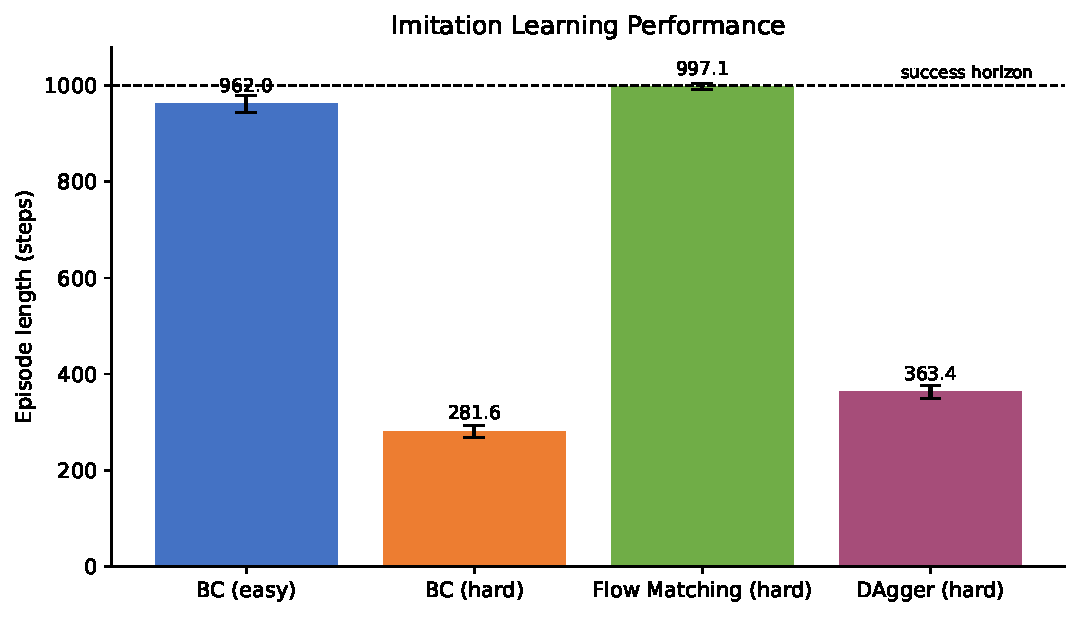
\includegraphics[width=\columnwidth]{method_comparison}
  \caption{主要方法的 episode length。误差棒为跨随机种子标准差，虚线为成功上限。}
  \label{fig:main}
\end{figure}

\begin{table}[t]
\centering
\caption{主要结果，均值$\pm$跨种子标准差。}
\label{tab:main}
\begin{tabular}{lcc}
\toprule
方法与环境 & Episode length & 机制 \\
\midrule
BC, easy & \BCEasyMean$\pm$\BCEasyStd & 单峰回归 \\
BC, hard & \BCHardMean$\pm$\BCHardStd & 均值坍缩 \\
Flow, hard & \FlowHardMean$\pm$\FlowHardStd & 多峰生成 \\
DAgger, hard & \DaggerHardMean$\pm$\DaggerHardStd & 在线重标注 \\
\bottomrule
\end{tabular}
\end{table}

图~\ref{fig:main} 与表~\ref{tab:main} 显示，BC 在 easy 模式上接近任务上限，
说明网络容量、动作块接口和优化过程正确。换到 hard 模式后，环境动力学并未改变，性能
却显著下降；结合动作分布图可把退化归因于标签多峰性，而不是一般性的训练不足。Flow
Matching 通过采样一个完整模式避免条件均值。DAgger 则利用闭环访问状态和一致专家标签，
同时处理多峰歧义与状态分布偏移。

\subsection{动作多峰性与优化收敛}
\begin{figure}[t]
  \centering
  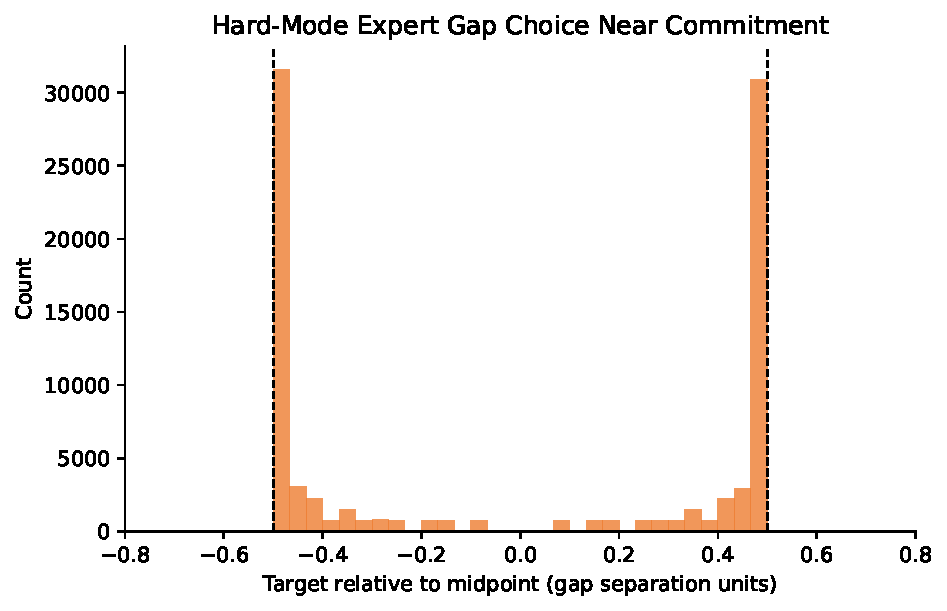
\includegraphics[width=\columnwidth]{hard_action_distribution}
  \caption{接近管道时 hard expert 的目标位置分布。两个峰对应两个合法缺口。}
  \label{fig:modes}
\end{figure}

\begin{figure}[t]
  \centering
  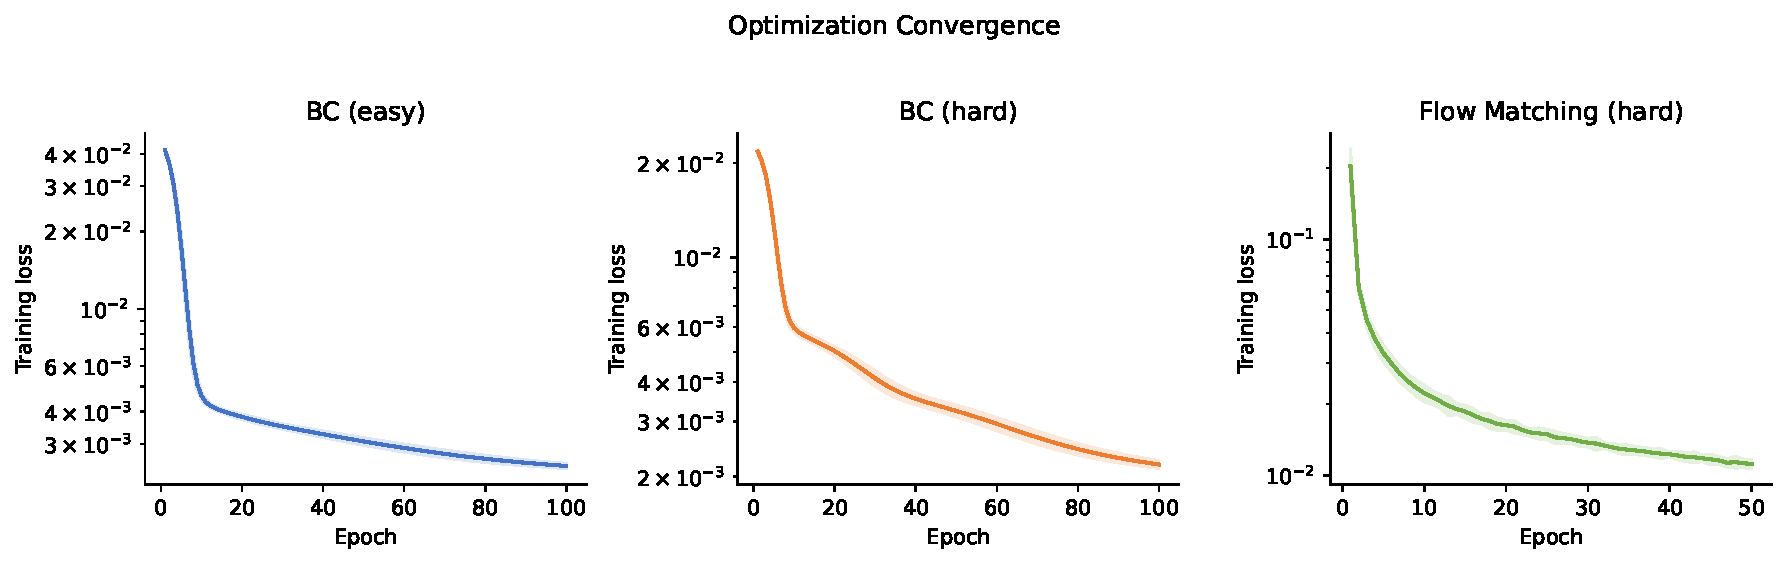
\includegraphics[width=\columnwidth]{training_curves}
  \caption{训练 loss 的跨种子均值与标准差。低监督 loss 不保证闭环控制成功。}
  \label{fig:loss}
\end{figure}

图~\ref{fig:modes} 给出 hard expert 的经验动作分布。MSE 可以持续下降，
但低 loss 只说明预测接近标签的二阶矩最优点；它不保证动作落入可执行模式。
图~\ref{fig:loss} 因而应与闭环指标共同解读。该现象也是面试中区分
``optimization error'' 与 ``objective mismatch'' 的典型案例。

\subsection{DAgger 学习曲线}
\begin{figure}[t]
  \centering
  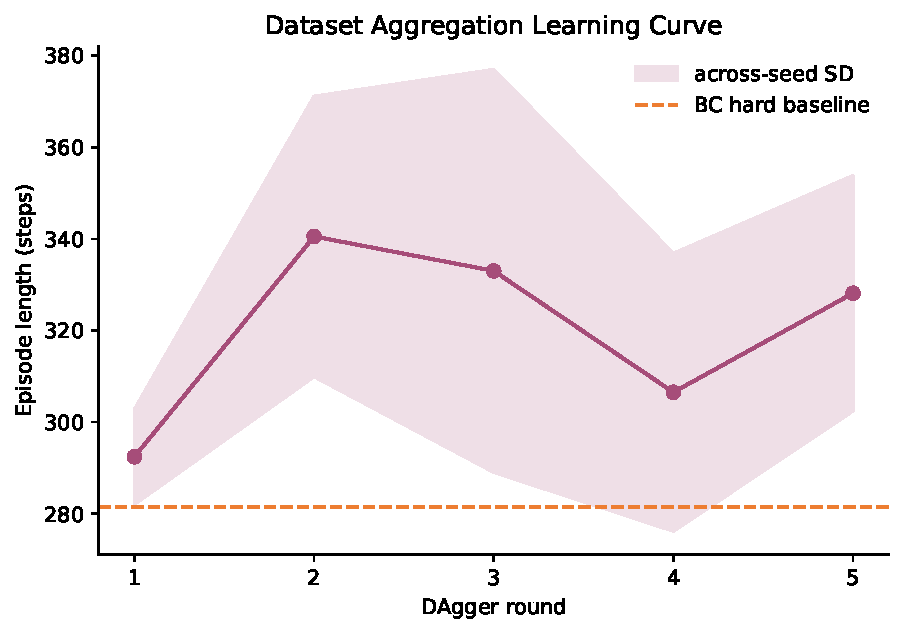
\includegraphics[width=\columnwidth]{dagger_learning_curve}
  \caption{DAgger 每轮评估结果。阴影表示跨种子标准差。}
  \label{fig:dagger}
\end{figure}

图~\ref{fig:dagger} 将性能变化与数据聚合轮次对应。每轮新数据来自当前策略真实访问的
状态，因而优先覆盖 BC 容易偏离的局部区域。曲线不必严格单调：新增状态改变数据分布，
有限 epochs 的重新训练也会引入方差。实践中应依据独立 validation rollout 保存最佳
checkpoint，而不是默认最后一轮最好。

\subsection{Flow Matching 的质量--时延权衡}
\begin{figure}[t]
  \centering
  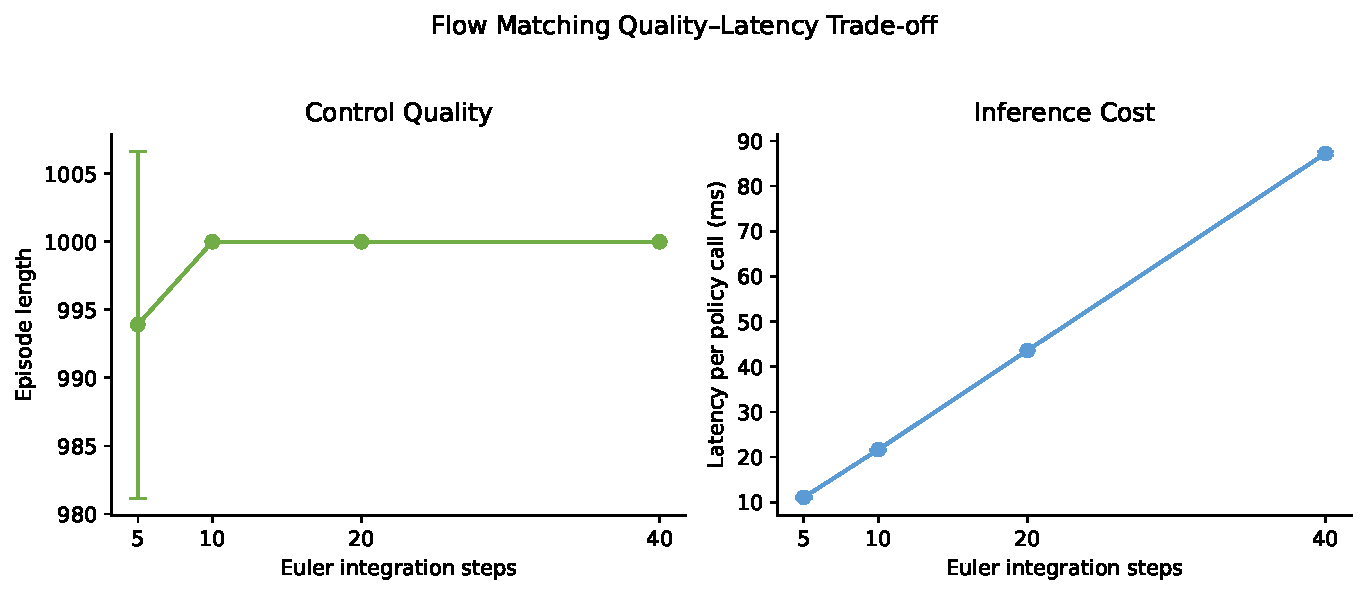
\includegraphics[width=\columnwidth]{flow_steps_ablation}
  \caption{Euler integration steps 对控制质量与单次查询时延的影响。}
  \label{fig:flow}
\end{figure}

Euler steps 增加会减小数值积分离散误差，但推理成本近似线性增长。
图~\ref{fig:flow} 用同一组模型权重和评价 seed 隔离 sampler 的影响。
若控制质量在某一点后进入平台区，继续增加步数只会提高延迟；部署选择应位于经验
Pareto frontier，而不是机械采用最大步数。

\subsection{重规划频率}
\begin{figure}[t]
  \centering
  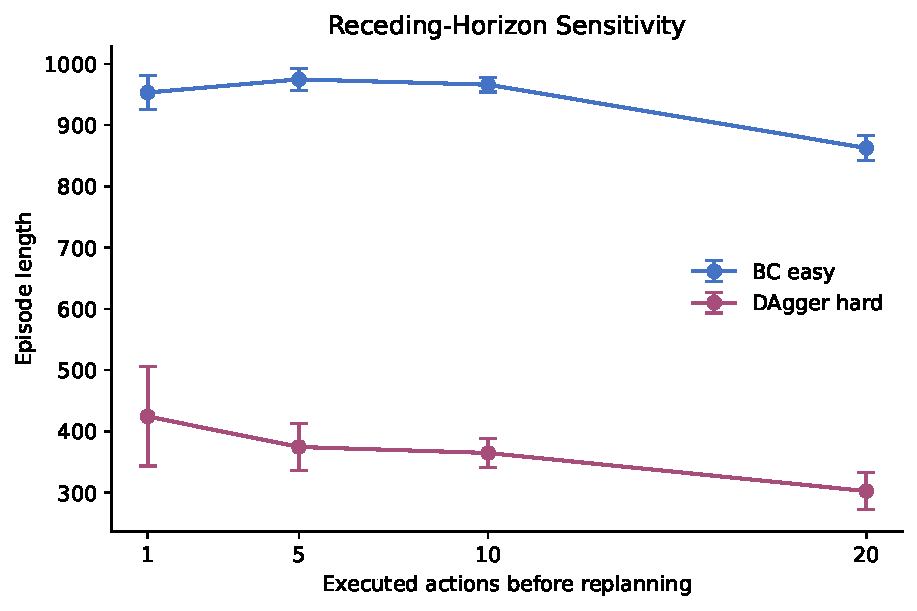
\includegraphics[width=\columnwidth]{execute_steps_ablation}
  \caption{执行动作数 $K$ 对 BC easy 与 DAgger hard 的影响。}
  \label{fig:chunk}
\end{figure}

$K=1$ 每一步重规划，反馈最频繁但查询开销最大；$K=20$ 完整执行 action chunk，
开环误差更容易累积。图~\ref{fig:chunk} 说明训练策略时应同时报告 horizon $H$ 与
execute steps $K$，否则“action chunk 长度”不足以定义部署行为。

\subsection{计算效率}
\begin{figure}[t]
  \centering
  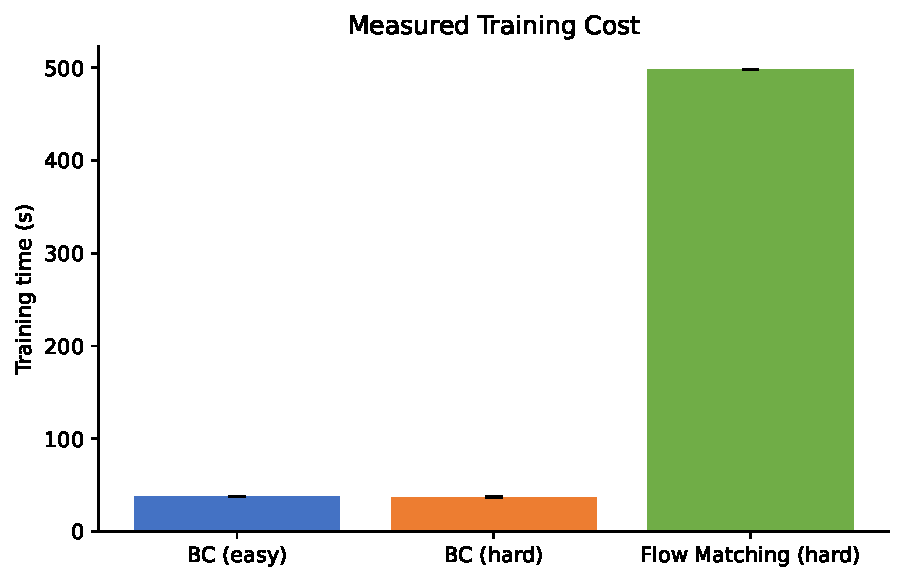
\includegraphics[width=\columnwidth]{training_efficiency}
  \caption{同一硬件上的实测训练时间。}
  \label{fig:time}
\end{figure}

BC 的 MLP 计算密度低，单进程难以饱和高端 GPU；本实验通过并行随机种子提高吞吐。
这种并行具有统计价值，因为它直接估计稳定性。相比之下，制造更大 batch 或无目的延长
epochs 虽可提高利用率，却会改变优化设定且不增加证据强度。

\section{误差来源与局限}
\textbf{环境规模。}Flappy Bird 只有四维观测，结论说明机制而非直接代表高维视觉控制。
\textbf{专家可查询假设。}DAgger 需要对 policy-visited states 获得专家标签；真实机器人
中这可能昂贵或存在安全风险。\textbf{随机专家与确定专家。}确定性重标注提高一致性，但
牺牲了多个合法策略的覆盖。\textbf{评价预算。}50 episodes 能估计大幅性能差异，对接近
上限的方法仍应给出 bootstrap confidence interval 或更多 episode。
\textbf{采样器。}本文只研究一阶 Euler 法；Heun 或自适应 ODE solver 可能得到更优
质量--时延折中。

\section{结论}
本实验展示了模仿学习中三个层次的问题。BC 在单峰离线数据上有效，但 MSE 无法表达
多峰动作分布；Flow Matching 通过条件生成建模修正输出分布；DAgger 进一步通过专家查询
修正策略访问分布。action chunking 将模型能力与系统闭环频率连接起来，必须通过端到端
rollout 而非仅监督 loss 评价。工程上最重要的原则是：明确数据分布、输出分布与部署分布
是否一致，并让每一项图表都能追溯到原始 episode 指标。

\section*{可复现性声明}
代码、单元测试、逐 seed JSON、抽样数据、绘图脚本、LaTeX 源文件与 PDF 均随仓库提供。
原始指标由实验程序直接写出，报告宏和图片由聚合脚本生成，不手工复制实验数字。

\bibliographystyle{plainnat}
\bibliography{../references}
\end{document}
